% v2-acmsmall-sample.tex, dated March 6 2012
% This is a sample file for ACM small trim journals
%
% Compilation using 'acmsmall.cls' - version 1.3 (March 2012), Aptara Inc.
% (c) 2010 Association for Computing Machinery (ACM)
%
% Questions/Suggestions/Feedback should be addressed to => "acmtexsupport@aptaracorp.com".
% Users can also go through the FAQs available on the journal's submission webpage.
%
% Steps to compile: latex, bibtex, latex latex
%
% For tracking purposes => this is v1.3 - March 2012

\documentclass[prodmode,acmtecs]{acmsmall} % Aptara syntax

% Package to generate and customize Algorithm as per ACM style
\usepackage[ruled]{algorithm2e}
\usepackage{tabularx}
\usepackage[justification=centering]{caption}
\renewcommand{\algorithmcfname}{ALGORITHM}
\SetAlFnt{\small}
\SetAlCapFnt{\small}
\SetAlCapNameFnt{\small}
\SetAlCapHSkip{0pt}
\IncMargin{-\parindent}

% Metadata Information
\acmVolume{9}
\acmNumber{4}
\acmArticle{39}
\acmYear{2010}
\acmMonth{3}

% Copyright
\setcopyright{rightsretained}

% DOI
\doi{0000001.0000001}

%ISSN
\issn{1234-56789}

% Document starts
\begin{document}

% Page heads
\markboth{M. Usman et al.}{A Survey of Gaming-as-a-Service models over Cloud Infrastructures}

% Title portion
\title{A Survey of Gaming-as-a-Service models over Cloud Infrastructures}

%%%%% Authors Here %%%%%
%\author{Muhammad Usman
%\affil{College of William and Mary}
%YAFENG WU
%\affil{University of Virginia}
%TING YAN
%\affil{Eaton Innovation Center}
%TIAN HE
%\affil{University of Minnesota}
%CHENGDU HUANG
%\affil{Google}
%JOHN A. STANKOVIC
%\affil{University of Virginia}
%TAREK F. ABDELZAHER

%\affil{University of Illinois at Urbana-Champaign}}
% NOTE! Affiliations placed here should be for the institution where the
%       BULK of the research was done. If the author has gone to a new
%       institution, before publication, the (above) affiliation should NOT be changed.
%       The authors 'current' address may be given in the "Author's addresses:" block (below).
%       So for example, Mr. Abdelzaher, the bulk of the research was done at UIUC, and he is
%       currently affiliated with NASA.

\begin{abstract}
Gaming as a service is an emerging application of Cloud Computing, where games can be hosted and distributed via cloud software services. This inherits the server-client models allowing sophisticated gaming software to run remotely on powerful servers and streamed to relatively simple devices. However, with the potential advantages, the service comes with research challenges such as limited network bandwidths, optimal service architectures, network jitters and connectivity problems causing loss in information being communicated across, to name a few. This survey discusses the various gaming as a service models and the research challenges in the field, discussing directions.

A game case study is deployed on AWS for studying the limitations
of the system and how to measure quality of experience from the players.
\end{abstract}


%
% The code below should be generated by the tool at
% http://dl.acm.org/ccs.cfm
% Please copy and paste the code instead of the example below.
%
\begin{CCSXML}
<ccs2012>
 <concept>
  <concept_id>10010520.10010553.10010562</concept_id>
  <concept_desc>Cloud Gaming~Gaming as a service</concept_desc>
  <concept_significance>500</concept_significance>
 </concept>
 <concept>
  <concept_id>10010520.10010575.10010755</concept_id>
  <concept_desc>Gaming on demand~Mobile Cloud Gaming</concept_desc>
  <concept_significance>300</concept_significance>
 </concept>
 <concept>
  <concept_id>10010520.10010553.10010554</concept_id>
  <concept_desc>Next generation mobile gaming~Online gaming</concept_desc>
  <concept_significance>100</concept_significance>
 </concept>
 <concept>
  <concept_id>10003033.10003083.10003095</concept_id>
  <concept_desc>Multimedia live streaming~Live video streaming</concept_desc>
  <concept_significance>100</concept_significance>
 </concept>
</ccs2012>
\end{CCSXML}

\ccsdesc[500]{Cloud Gaming~Gaming as a service}
\ccsdesc[300]{Gaming on demand~Mobile Cloud Gaming}
\ccsdesc[100]{Next generation mobile gaming~Online gaming}
\ccsdesc[100]{Multimedia live streaming~Live video streaming}

%
% End generated code
%

\terms{Cloud Gaming, client-server architecture models, quality of experience, Cloud Computing, Distributed Computing}

\keywords{cloud, game, video, remote}

\acmformat{Gang Zhou, Yafeng Wu, Ting Yan, Tian He, Chengdu Huang, John A. Stankovic,
and Tarek F. Abdelzaher, 2010. A multifrequency MAC specially
designed for  wireless sensor network applications.}
% At a minimum you need to supply the author names, year and a title.
% IMPORTANT:
% Full first names whenever they are known, surname last, followed by a period.
% In the case of two authors, 'and' is placed between them.
% In the case of three or more authors, the serial comma is used, that is, all author names
% except the last one but including the penultimate author's name are followed by a comma,
% and then 'and' is placed before the final author's name.
% If only first and middle initials are known, then each initial
% is followed by a period and they are separated by a space.
% The remaining information (journal title, volume, article number, date, etc.) is 'auto-generated'.

\begin{bottomstuff}
Author's addresses: G. Zhou, Computer Science Department,
College of William and Mary; Y. Wu  {and} J. A. Stankovic,
Computer Science Department, University of Virginia; T. Yan,
Eaton Innovation Center; T. He, Computer Science Department,
University of Minnesota; C. Huang, Google; T. F. Abdelzaher,
(Current address) NASA Ames Research Center, Moffett Field, California 94035.
\end{bottomstuff}

\maketitle


\section{Introduction}

Cloud computing has been accepted as a new computing paradigm which has introduced a different concept resources being offered ‘as-a-service’ to the consumer needs. The basic concept of Cloud Computing is the provision of computing resources (hardware, software and network infrastructure) and services through the internet medium. These resources and services are maintained by third party organizations on the internet, reducing the cost of maintenance and management of hardware and software to the consumer or client companies and individuals. These third parties are also responsible to keep the data available, accessible and protected at all times. Third parties provide their resources (storage, processing, application and network) to the cloud clients (individual and companies) on and according to their demand on lease as specified in the Service level agreements (Misra,). Due to the sheer nature of Cloud computing, where it provides many advantages to unlimited space, it presents challenges on data protection and needs for secure accessibility. Industry standards have produced risk standards for cloud computing security (NIST, KIRAN) looking at the environments as a whole.

Recently another area of study has emerged as a merger of cloud computing and video gaming, known as ``Cloud Gaming'' or ``Gaming as a service (GaaS)''. In cloud gaming, games are executed on the cloud and their high definition scenes are rendered using intensive cloud machines. After running the games remotely, output of the games, in the form of video frames, is streamed back towards the client. Similarly, user’s interaction with gaming application is sent back to the game running on cloud over the Internet \cite{cai2014toward}, \cite{gharsallaoui2014comparative}, \cite{shea2013cloud}, \cite{cai2013next}, \cite{chuah2014cloud}, \cite{wang2012cloud}, \cite{huang2013gaminganywhere}.

 Figure \ref{img:gamingApp} is explaining the working mechanism of a generic cloud gaming application.
\begin{figure}[h]
  \centering
  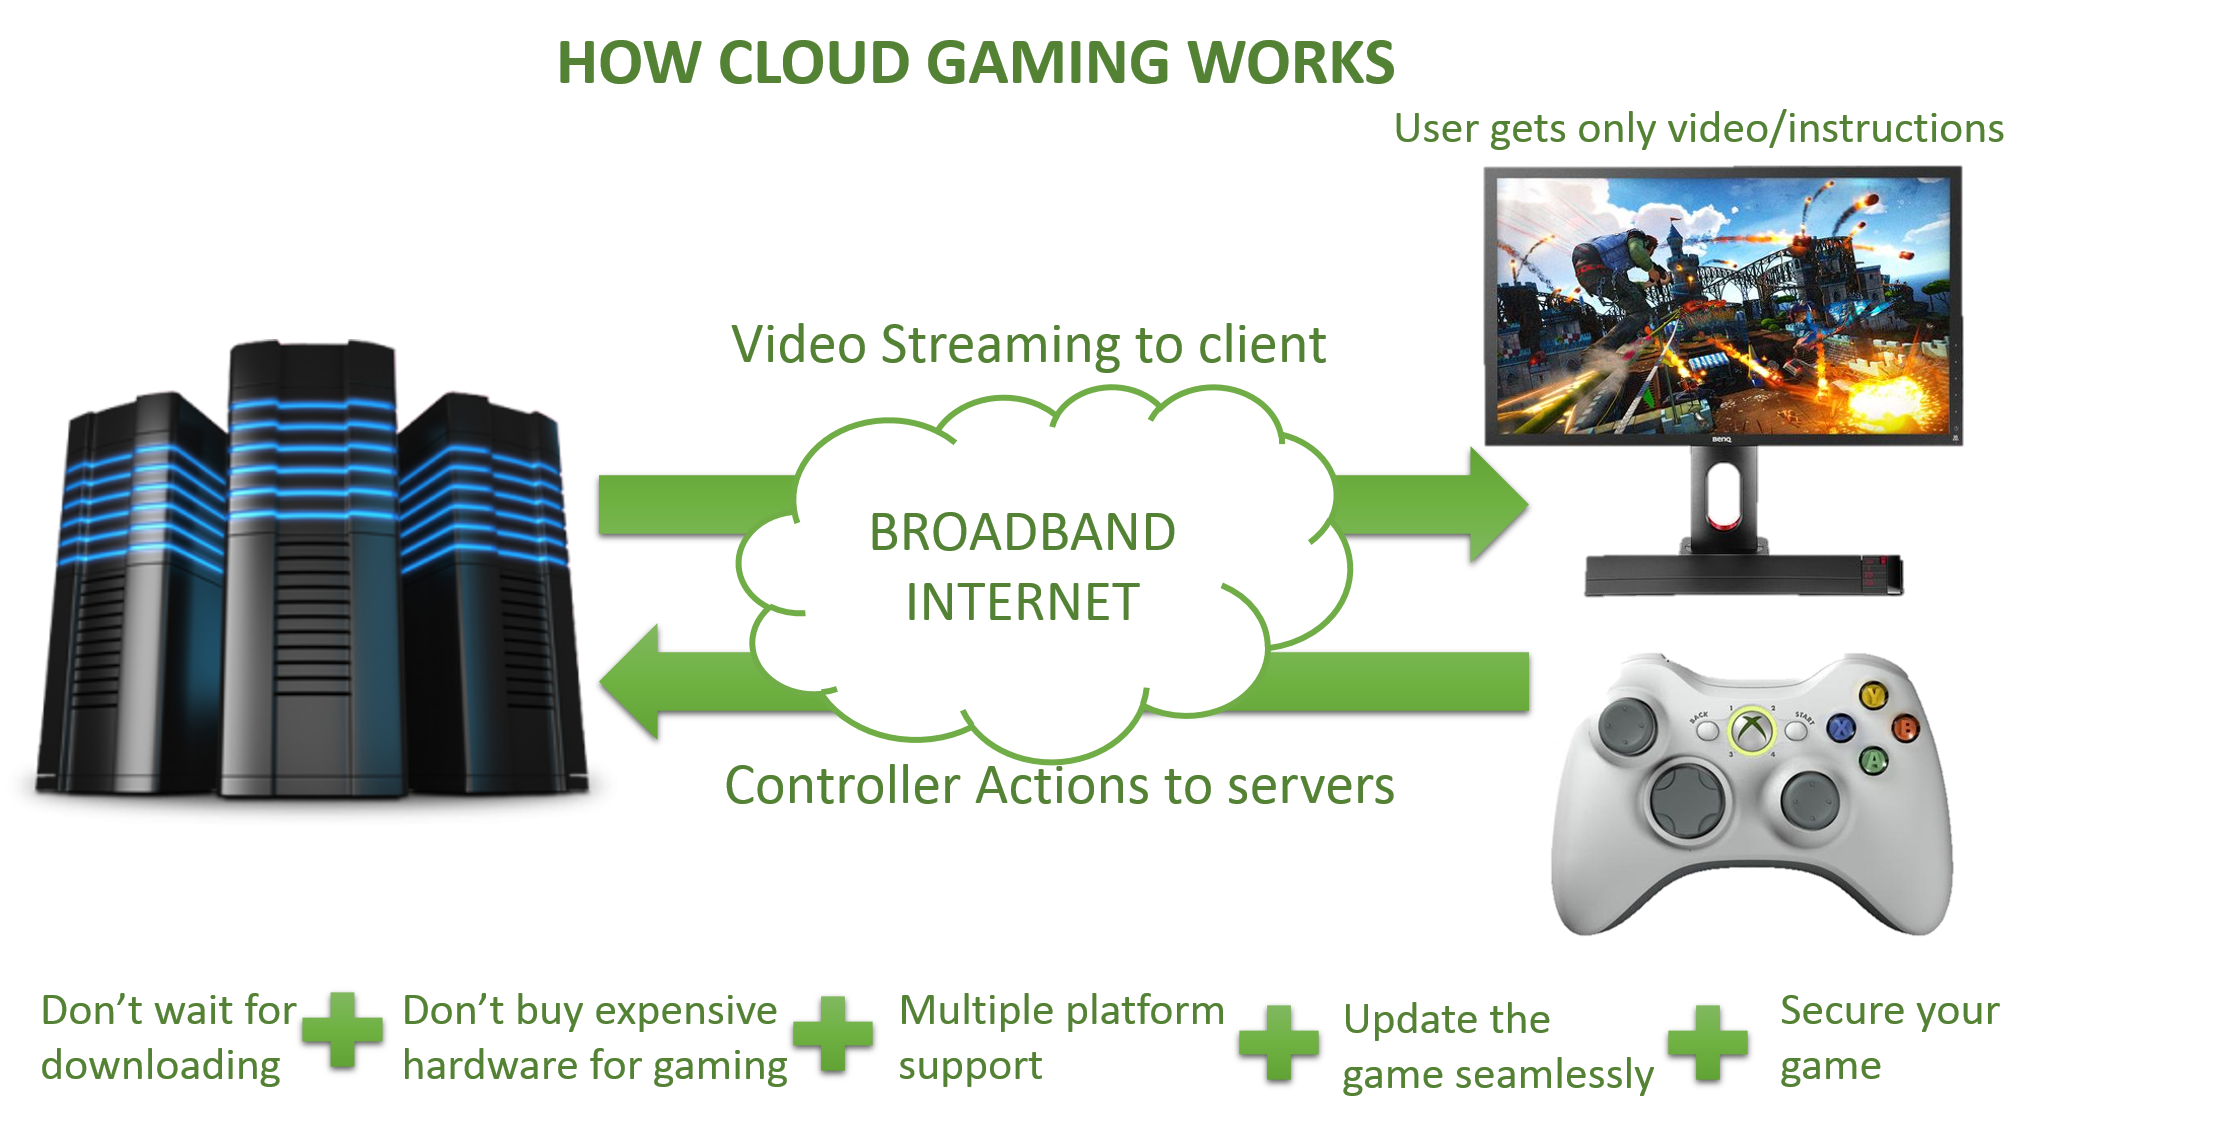
\includegraphics[width=5in, height=2.5in]{../../Report_Images/Picture3.png}
  \caption{General Cloud Gaming Application}
  \label{img:gamingApp}
\end{figure}


This technology has made it easier for the end users to play intensive games on a thin client without updating software or hardware of their machines.




\section{Motivation and Scope}
Cloud Gaming is now a well known area of Cloud Gaming witnessing significant progress over the years yet there is no decent recent survey of the domain. There exist some good introductory surveys such as [Towards Gaming as s Service, IEEE Internet Computing, 2014] but are now outdated with respect to state of the art. There are some more recent studies which are relevant but not in depth. For instance [A Survey of Interactive Remote Rendering Systems, Computing Surveys 2015] primarily covers interactive rendring system but it also has a chapter on cloud gaming. Similarly there are some other surveys which provide some overview of the domain but do not cover it in detail such as [Mobile Cloud Gaming: Issues and Challenges (2013) and Next generation mobile cloud gaming (IEEE SOSE 2013)]. This warrants the need of a survey which covers state of the art in all areas pertaining to Cloud Gaming.

In this survey, we investigate different cloud gaming techniques and then analyse them by filtering them in relevance to the cloud computing paradigm and improving gaming experience for players. The mentioned new technology provides many advantages to the players as well as to the developer community of the computer games

The main goals of this survey are as follows:
\begin{itemize}
\item	Introduce a system review of cloud gaming
\item	Literature review of gaming algorithms and architectures
\item	Provide an overview of existing models in the context of supporting cloud computing concepts.
\item	Highlight existing research areas and future challenges in this area of cloud gaming.
\end{itemize}

\subsection{Key Challenges}

QoS and QoE definition\\
player experience

\subsection{Overview of this Survey}

\section{Cloud Gaming in Literature}


Cloud gaming provides the following advantages to the player community of computer games \cite{cai2013next}:
\begin{itemize}
  \item \textbf{Thin Client:} A very thin client is needed to play the game, as games are being rendered on the cloud, and video is streamed from server. As a result, the client is required to receive and show the video frames of the game, and send the user's interactions to the cloud.
  \item \textbf{Potential Battery Conservation:} Complex rendering is being done on the cloud which reduces the battery consumption of the client machine.
  \item \textbf{Seamless gaming:} Games are platform independent and the players can seamlessly play the same game resuming from the same level by sitting anywhere in the world.
\end{itemize}

\subsection{Involved Actors}

Players

Developers:
Apart from being beneficial for the player community, cloud gaming provides following advantages to the developer community of computer games:
\begin{itemize}
  \item \textbf{Secure Gaming:} Data related to the game (e. g. level information) is residing in the cloud and only developer has complete access to all the data. This stops the users from getting the pirated version of the game.
  \item \textbf{Easy Updates:} Game logic and game information are mostly residing on the cloud so the developer can update the cloud part of the game and that would be automatically reflected to the client.
  \item \textbf{Unlimited Cloud Resources:} Developers have no need to worry about the storage or computing resources for the game as the cloud is providing scalable resources\cite{cai2013next}.
\end{itemize}

\subsection{Cloud Gaming Challenges}
Despite the advantages provided by cloud gaming, the area still has many challenges which are needed to be managed by the researchers. The challenges faced by the cloud gaming application depend on the architecture of that application. For example, the biggest hurdle in the efficiency of a `Remote Rendering Cloud gaming application' is \textbf{the limited bandwidth}. Since the scenes of the game have to be transmitted over the internet in the form of video frames. Therefore, the bandwidth needs to be fast enough to quickly transmit these frames to the client and interactions of client back to the server. Similarly, the complication in `Local Rendering application' is the \textbf{formation of such instructions} that could be used to completely render the scene of game at client side.\cite{cai2014toward}
Other than these obstacles, rendering the game remotely with efficient encoding is also considered as a problem in this technology. Moreover, recent happening with Onlive and GaiKai has guided the researchers to think about a better business model that can be used by cloud gaming service providers.

\section{cloud computing}
The National Institute of Standards and Technology-(NIST) defines Cloud Computing as a “model for enabling ubiquitous, convenient, on-demand network access to a shared pool of configurable computing resources (e.g., networks, servers, storage, applications, and services) that can be rapidly provisioned and released with minimal management effort or service provider interaction” (Mell, 2011). Cloud computing provides a virtual computing environment with scalable and elastic computing services in accordance with the demand by consumers.
The Cloud computing paradigm argues to offer a number of benefits such as – flexibility, trust, cost effectiveness, reliability, provision of software updates, pay-as-you-go, reduced disaster recovery cost, remote access, secure and adoptable. A cloud client can access cloud services using their desktop computers, laptop computers, tablets and mobile phones, equipped with internet connection facilities through simple web clients. As described by (Wyld, 2009) cloud computing offers, with further potential of:
-	Rapid scalability and deployment capabilities (to provide ‘just in time’ computing power and infrastructures).
-	Decreased maintenance and upgrades for individual software maintenance.
-	Improved resource utilization such as elasticity, flexibility, efficiency.
-	Improved collaboration capabilities for software.
-	Ability to engage in usage-based pricing, making computing a variable expense, rather than the traditional fixed capital cost with high overhead.
-	Reduced information technology infrastructure needs for upfront and support costs
-	Capacity for on-demand infrastructure and computational power
-	Ecofriendly with a green or reduced environmental footprint
-	Improved disaster recovery capabilities through fault tolerance mechanisms.
Figure 2 Cloud Computing c.f. (Srinavasin, 2012) (REDRAW)

The recent NIST definition of Cloud Computing (L. Badger, May 2011) offers five main characteristics of Cloud computing most beneficial to clients:
-	Users can automatically benefit from the Cloud services without communicating with the service providers.
-	Standard protocols are used to access the computing resources over the network.
-	Cloud services follow a multi-tenant model allowing resources to be pooled and shared among users.
-	Computing capabilities can be quickly scaled in or out based on the users’ varying demands.
-	Users pay for utilized computing capabilities based on a pay-per-use model.
\subsection{Cloud Computing Delivery Models}
Cloud computing providers offer their services in three different models.
Diagram for models windowns azure pre

Software as a Service (SaaS): SaaS delivery model has introduced the concept of “software as service”. The software (applications) run on the cloud (located at the provider’s servers) and the service consumers can access these via the Internet, working on the software application as if it was hosted locally on their machines. Consumers do not need to know about the infrastructures that run the applications and only have to pay for the time and consumption of resources during this time (Mell, 2011),(Rittinghouse J, 2010).
Platform as a Service (PaaS): PaaS provides affective environment and powerful tools for developers to create and deploy the applications. Developers do not need to know any details about infrastructure underlying this service such as networks, operating systems, storage. Thus, the developers or company focus on innovation instead of worrying about the infrastructure problems. Google App En-gine is a good example for this service (Buyya, 2011) (Mell, 2011).
Infrastructure as a Service (IaaS): IaaS considered the basic layer of computing resources. It provides on demand and scalable full infrastructure resources (e.g. servers, software, network equipment and storage). IaaS enables consumer to manage and configure the cloud servers similar to the ordinary physi-cal servers. With IaaS, consumer will get rid of problems of purchasing the latest technolo-gy, maintenance, upgrading of software and software licenses. Elastic Compute Cloud (EC2) from Amazon is a sample of IaaS (Buyya, 2011) (Rittinghouse J, 2010).


\subsection{Gaming on the Cloud}
It is inferred that the idea of Cloud Gaming was emerged from the concept of audio and video streaming \cite{mungee1999design}. In 2006, De Winter et al. \cite{DeWinter:2006:hybridThinClient} proposed a hybrid thin client protocol for multimedia streaming where they addressed interactive games too. In their work, a realtime desktop streamer was formulated using a video-codec to stream the graphical output of applications after GPU- processing to a thin-client device. Then, in 2007, Eisert and Fechteler \cite{eisert2007remoteRendering} introduced the concept of remote rendering of computer games. This work was a part of European project Games@Large \cite{tzruya2006gamesATlarge} and can be declared as a stepping stone in cloud gaming. Apart from elaborating the concept of rendering the game scenes at server and streaming the video scenes towards the client, the work also explained the idea of local rendering for cloud gaming application where graphic commands were streamed to the client and game scenes were rendered locally. Also, a closer step to this fascinating technology was taken by Eisert and Fechteler\cite{eisert2008LanGaming} in 2008 when they introduced the idea of computer graphics streaming over Local Area Network (LAN). The work was specifically focusing on graphics in video games and how these games can be streamed over the local area network. In 2008, emergence of OnLive\cite{onlive} as the first commercial platform for providing 'Gaming as A service' and its high appreciation motivated the business and academic community to take 'Cloud Gaming' more seriously. After this progress, most of the work was done to overcome the challenges (Bandwidth usually) in CG. After OnLive, many other cloud gaming platforms also emerged including Gaikai\cite{gaikai}, NVIDIA GRID\cite{nvidia}, and GamingAnyWhere\cite{huang2013gaminganywhere} which was the first open source cloud gaming platform that has been started to use for research purpose. Most of the cloud gaming platforms are using remote rendering model of CG and game video is being streamed towards the client. But, an important break-through was done by Wei Cai et al. in \cite{cai2013cognitive} when they proposed and implemented a `Cognitive Model' of CG in which game components were being transferred from the cloud to the client and vice versa to get a better gaming experience.

\section{Gaming Architectures}
Recent literature describes two kinds of cloud gaming \cite{hong2015enabling}:
\begin{enumerate}
  \item \textbf{Video Streaming Cloud Gaming:} Most appreciated form of cloud gaming in which video is streamed towards the client. It is usually referred as `Gaming on Demand' and in the following sections, the term Cloud Gaming would be used instead of Video Streaming Cloud Gaming.
  \item \textbf{File Streaming Cloud Gaming:} In this form of cloud gaming, a portion of game application is downloaded at the client side to start the game. Once the game is started on client side, the remaining file is downloaded on the fly. Kalydo is one of the companies which use this kind of cloud gaming service \cite{kalydo}.
\end{enumerate}

\subsection{Application Components}
Since, in cloud gaming, output of games is streamed to client over the internet and users' interactions are sent back towards the cloud. Therefore, to do all these functions, a cloud gaming platform mostly have specific components and each of them does its part and forwards its output to other. A general online game would be having four main components\cite{cai2014toward}:
\begin{itemize}
    \item	Input module
    \item	Game logic
    \item	Networking module
    \item	Rendering module
\end{itemize}

Based on these components, different architectures are possible for a cloud game. Firstly, these components and their functionality will be explained and then the possible architectures of a cloud gaming application will be analyzed.

\subsubsection{Video Renderer}
Once the input commands are received by the game logic, game world changes according to inputs provided by the player. Then, video rendering unit renders the updated game frames using graphical processing unit (GPU). Another method used for generating frames of game scenes is to let the game render its video frames and take a snapshot of the game desktop by desktop capture module at a specified frequency. This method is used in one of the two implementations of video source by GamingAnywhere platform. Also, depending on the operating system of the end user, audio of the game is generated by the audio source of the system. For example, GamingAnywhere uses ALSA library for Linux, and Windows session audio API for Windows to capture the audio\cite{gharsallaoui2014comparative}.

\subsubsection{Input Handler}
User interactions are received by this module. After receiving the inputs, the module converts these mouse clicks and key strokes to appropriate commands and send those commands to the game logic. This component must be at the client side of a cloud gaming system\cite{shea2013cloud}.

\subsection{Possible Architectures of Cloud Gaming Applications}
Recent literature provides two different parameters for elaborating CG application architectures as described below:
\begin{enumerate}
  \item Models with respect to components' division between client and server
  \item Models with respect to game integration with Cloud Gaming platform
\end{enumerate}

\subsubsection{Architecture w.r.t Components' Division}
The first approach is discussed in \cite{cai2014toward}, and according to this work, a cloud gaming application could be distributed amongst the client and the server of the game. These different distributions of components are referred as architectures of a cloud game. Based on the mentioned components, possible architectures are \cite{cai2014toward}:

\begin{table*}[h]
    \centering
  \begin{center}
  \begin{tabularx}{\textwidth}{|p{3cm}|p{4cm}|p{5.5cm}|}

  \hline
  % after \\: \hline or \cline{col1-col2} \cline{col3-col4} ...
    \centering Cloud gaming model & \centering Components of game at Client & \centering Components of game at Cloud                 \tabularnewline \hline
    \centering Remote Rendering & \centering Input Controller & \centering Game Logic, Networking, Database, Video Renderer          \tabularnewline  \hline
    \centering Local Rendering & \centering Input Controller, Video Renderer & \centering Game Logic, Networking, Database           \tabularnewline  \hline
    \centering Cognitive & \centering Dynamically decided & \centering Dynamically decided                                           \tabularnewline  \hline
    \end{tabularx}

    \end{center}

    \caption{Different Models of Cloud Gaming}
    \label{tab:models}

\end{table*}

\begin{enumerate}
  \item \textbf{Remote Rendering:} This model is the ultimate inverse of a local (stand-alone) gaming application. The function of the client in this architecture is just to receive inputs from users, convert those inputs to commands and send those commands to the game residing in the cloud. On the other hand, all the remaining components of the game are residing in the cloud. The architecture works in such a way that whenever a user interacts with the gaming application, input commands are generated and sent over the internet to the game logic using input controller. Then, game scenes are updated and actions are taken using game logic and video rendering unit render scenes as frames. After that, these frames are sent to the client over the internet\cite{barboza2010simple}. The model provides smart solution for the users not having sufficiently intensive hardware to render the graphics of high definition games. But, this can be clearly observed that the bottleneck would be ``Bandwidth'' in this scenario, as the Internet is playing a key role here.

  \item \textbf{Local Rendering:} The model does components' divisions in such a way that video renderer also resides at client side with input controller, and remaining parts of the game are kept in the cloud. The model resolves the bandwidth issues by rendering the scenes at the client side. This architecture resembles with remote rendering model till the input commands update game scenes, but rather rendering the scenes and sending the packets, output instructions are generated and sent towards the client. Then, the client receives these instructions, renders the scenes using these instructions and displays to the end user\cite{cai2014toward}. As mentioned, in comparison to remote rendering, this model is remarkably efficient in terms of internet bandwidth. Mobile browser gaming has adopted this architecture in most of the applications.

  \item \textbf{Cognitive:} This model has dynamic separations of client and cloud parts of the game. In this approach, client and cloud divisions of the game are dynamically decided on behalf of the user resources (e. g. computation and rendering power, bandwidth). Cai et al. (2013) \cite{cai2013next} proposed this method in their work where cloud gaming application was divided into various parts. Also, the application was able to transfer game components from cloud to the client and vice versa. But, to achieve this collaboration (on-loading and off-loading components), the application must be partitioned into components in such a way that can resolve dependency issues. Also, the work did not elaborate the control mechanism of this components' movement, there should be a component within the application that can make decisions on this on-loading and off-loading actions.
\end{enumerate}


\subsubsection{Architecture w.r.t Game Integration with Platform}
The work described in \cite{cai2016future} distributes cloud gaming applications in three different architectures based on how games are integrated with the cloud gaming platforms. Details of these models are as follows:
\begin{enumerate}
  \item \textbf{Black-box:} In these type of cloud gaming applications, game scenes are rendered in cloud and are streamed back towards the client.
  \item \textbf{In-Game Context:} These applications are programmed in such a way that game streaming is made adaptive with using some optimization techniques.
  \item \textbf{New Programming Paradigm:} In this architecture, gaming application is distributed between the game client and server.
\end{enumerate}

\subsection{Quality Parameters}

\subsection{Bandwidth}
\subsection{Connectivity}
\subsection{Security}
\subsection{Player Experience}
\subsection{Lack of development platforms}
\subsection{QoS/QoE}
\subsection{Rendering}

\section{Current Cloud Gaming Platforms}
Cloud gaming has been able to grasp the attention of entrepreneurs, that is why various companies are providing ``Gaming as a Service''. Some of the notable cloud gaming platforms are discussed here:

\subsection{GamingAnyWhere}
GamingAhyWhere is an open-source cloud gaming platform that provides reconfiguration for researchers and developers. Huang et al.(2014) suggested that each component of this video streaming system can be replaced by another component having different protocol or algorithm. Also, their work elaborated the flow of clients’ communication with game servers and portal servers. Portal server provides an interface to the user for login to a system and selecting the desired game. When the user selects a particular game, the portal server finds and launch that game on a server, and sends the URL of the game server to user. The client connects to the game server and starts playing game \cite{huang2014gaminganywhere}.

\subsection{OnLive}
OnLive is a real time video streaming platform for cloud gaming and its clients are available for various operating systems. The platform lies in the category of video streaming platforms of online gaming as scenes are rendered virtually and streamed back to the thin client\cite{gharsallaoui2014comparative}. Due to its robust structure and real-time compression techniques, it had been able to get noticed by the business community and Sony has acquired this platform in 2015\cite{onlive}. Manzano et al.(2014) identified three phases of an OnLive session and this explains the overall flow of client's interactions with the cloud gaming application\cite{manzano2014dissecting}:

\begin{enumerate}
  \item User authentication and allocating the user a particular site for load balancing
  \item OnLive main menu
  \item Game playing
\end{enumerate}

To elaborate their work\cite{manzano2014dissecting}, in the first phase of communication, a user connects with the OnLive authentication server and it is authenticated possibly using HTTP-based messages. Once the user is authenticated, it probably (communication between client and authentication server is encrypted) gets the IP of onLive servers present at more than one locations. Then, client measures its round trip time (RTT) with those servers to find the most suitable one for it to make a connection. After finding the closest server, the client identifies available downstream bandwidth using another measurement session and with the help of RTT and calculated downstream, client adjusts its streaming bit-rate that can also be changed during streaming. In phase two, the client communicates with OnLive main menu server and main menu which is an interactive video, is streamed back towards the client using the same protocol that would later be used for game streaming. Using this menu, player selects a game for playing and this phase ends when the desired game is selected. Finally, communication between client and OnLive gaming server gets started and the game is streamed towards the thin client.

\subsection{StreamMyGame}
This platform provides some extra features apart from cloud gaming services to the users. Using this system, users can record their game-play videos and upload that recorded video to Facebook, Youtube, and other sites. Also, clients can broadcast their videos to the local network and can communicate with other members using community services. \cite{gharsallaoui2014comparative}


\subsection{Amazon AppStream}
AppStream service provided by Amazon Web Services (AWS) is typically designed to stream the output of a particular application. After executing the application on a virtual machine of the service, resultant output of the execution is streamed towards the client. Though this service is not especially formulated for game streaming but recently its focus has been shifted to the cloud gaming and by introducing its SDK in Java language, it does provide the capability of \textbf{Hybrid Streaming} to the developers.\cite{appStream}

\section{Current Game Genre}
Depending on some specific parameters, current games are usually categorized in different game classes, and these classes are usually referred as `Game Genres'. Due to diversity in the games, analyzing them with respect to different parameters (e. g. Game-play, camera-view, purpose et cetera) yields different genres. For example, Lee et. al (2014) have used different parameters to classify the games in various genres. Table \ref{tab:gamegenre} is showing some of their classification work \cite{lee2014facet}:
\begin{table*}[h]
    \centering
    \begin{center}
    \begin{tabularx}{\textwidth}{|p{4cm}|p{9cm}|}


      \hline
      % after \\: \hline or \cline{col1-col2} \cline{col3-col4} ...
      \centering Parameter Used & \centering Game Genre Classification  \tabularnewline \hline
      \centering Game-play & \centering Action, Action/Adventure, Racing, Fighting, Puzzle, Role Playing, Shooting, Simulation, Sports, Strategy \tabularnewline \hline
      \centering Point-of-view & \centering First Person, Third Person, Overhead, Multiple perspectives  \tabularnewline    \hline
      \centering Purpose & \centering Education, Entertainment, Exercise, Meditation, Party, Social  \tabularnewline        \hline
      \centering Presentation & \centering 2D, 3D, Isometric, Static Background, Vertical Scrolling, Side Scrolling, Grid Based, Perspective manipulation  \tabularnewline  \hline



    \end{tabularx}
    \end{center}
    \caption{Different Game Genres}
    \label{tab:gamegenre}

\end{table*}

It can be seen in Table \ref{tab:gamegenre} that the resultant game genres will be depending on the chosen parameters for classification.


\subsection{Effect of Game Genre on Cloud Gaming Experience}
The recent research has found that `Cloud gaming' is not equally appropriate for each of the current game types. Generally, genres that have drastically changing consecutive frames are considered to be less appropriate to deploy as cloud gaming applications. To look deeper into the problem, study is done to analyze the different game types in terms of their scenes complexity, as it does play a major role in deciding game's friendliness for the cloud. For example, to analyze the motion and scene complexity of games, Claypool (2009) \cite{claypool2009motion} studies the different game classes by using game perspective (Camera view) as the parameter of classification. After identifying four different game types (First Person Linear (Battlefield), Third Person Linear, Third Person Isometric, and Omnipresent), motion and scene complexity for each of the game class is computed. The results of their work have found that `First Person games' have higher motion (PFIM = Percentage of Forward/backward or intra-coded Macroblocks) than Omnipresent and Third Person Linear games, and Third Person Isometric games are having the lowest PFIM. Also, Omnipresent games are observed to have the highest scene complexity, and Third person Linear and First Person games are considered to have the least complex scenes.

Likewise, the difference in Gameplay and overall structure of the game also influences the rate of delay tolerance and delay sensitiveness. Domineco (2014) \cite{domenico2014evaluation} has described the effect of game genre on sensitiveness. In the proposed work, the author discusses four game types including Action games, Racing games, Real-Time Strategy (RTS) games, and Puzzle games. Using OnLive as a cloud gaming platform, experiments are conducted on games from each of the mentioned genres, and it is seen that Puzzle and RTS games are more delay-tolerant as compared to Action and Racing games. The reason for this change is that, in later games, complex synchronization over the network is required to determine the collision between game objects after player's interactions. On the other hand, RTS games feature lots of interactions for which the resultant can be computed locally without synchronizing with the server.


\subsection{Cloud Friendly Game Genre}
Some of the recent studies are specifically done to classify the current game genres with respect to their cloud friendliness. For instance, Lee et al. (2012) \cite{lee2012all} propose a model to predict the suitability of a particular game to be deployed on the cloud. The suggested model investigates the effect of response latency on users' experience for three game types (First Person Shooting (FPS), Role Playing (RPG), Action). To illustrate, the work analyzes spatial and dynamic changes on the screen for these games, and how frequently the game demands input from the user. Using this model, Action games are found less susceptible to latency and have lower real-time strictness than FPS and RPG games. The reason for this is, in Action games, the users mostly have to provide many inputs for certain attacks, and these attacks last for more than 3 seconds and cause a damage.

Another study is conducted by Suznjevic et al. (2014) \cite{suznjevic2014towards} in which change in subsequent frames is observed. The study suggests that Shooting and Action games are more dynamic and their temporal metrics have the highest values. Therefore, these games can be referred as `un-appropriate' for cloud.

\section{Solutions Discussed in Previous Work}
The basic obstacle in achieving better quality of experience in cloud gaming is its heavy dependence on network bandwidth \cite{lampe2013will}. Most of the commercial cloud gaming services including OnLive, StreamMyGame, and GaiKai are using `Remote Rendering Model' of Cloud Gaming which makes it difficult to use in low bandwidth areas. Therefore, studies have been conducted to reduce quality of experience issues at user end. Solutions can be divided in following categories:
\begin{itemize}
  \item Using adaptive streaming technique \cite{hong2015enabling},\cite{ahiska2012adaptive},\cite{wu2015enabling}
  \item Applying cognitive model for Cloud Gaming \cite{cai2015cognitive},\cite{cai2014decomposed}
  \item Enhancing video encoding at server side \cite{shi2011using}
  \begin{itemize}
    \item Video encoding optimization using graphic rendering contexts \cite{shi2011using}
    \item Efficient encoding using game engine information \cite{semsarzadeh2014video}
  \end{itemize}
  \item Frame Prediction \cite{lee2015outatime},\cite{lee2014demo}
  \item Peer assisted Cloud Gaming \cite{cai2014cloudlet},\cite{cai2012multiplayer}, \cite{suselbeck2009peer}
\end{itemize}

(We can discuss each of these solutions in detail too)

\section{Cost Efficient Solutions for Service Providers}
In the past, most of the studies were focused on enhancing the quality of experience of end user (Game player). But, one of the most important entity in the Cloud Gaming technology is the service provider. The one who is providing cloud gaming services to the end user. Recently, one of the widely praised service provider of Cloud Gaming, OnLive, has shut down its services and sold its patents to Sony \cite{cai2016future}. These kind of events encouraged researchers to work on cost-effective cloud gaming for the service provider. Rendering the gaming application at cloud servers put a lot of load at server side and sending those scenes towards the client also require investment on the network bandwidth. Therefore, studies are done to find solutions for Cloud Gaming Service Providers (CGSPs). For instance, Hong et al. \cite{hong2013qoe} investigated the optimum use of virtual machines at cloud gaming servers to give maximum profit to the service provider. Similarly, in the work of Tian et al. \cite{tian2015achieving}, to minimize the overall cost of CGSPs, adaptive use of resources is proposed from three different angles: (a) Adaptive Data Center Selection; (b) Adaptive virtual machine allocation; and (c) Adaptive Video bit-rate configuration. To consider all the factors involving in an optimum solution, a constrained stochastic optimization problem was formulated and Lyapunov optimization theory was applied to derive a cost effective online strategy. Likewise, `Cloud Resource Minimization' specifically in the case of Cognitive model of Cloud gaming is done in the work proposed by Cai et al.\cite{cai2014resource}. In the proposed system, cloud resource monitoring in real-time is done and components of the game are dynamically transferred to selected terminals to reduce its own resource consumption.


\section{User Quality of Experience (QoE) Studies}
Measuring user quality of experience in the case of cloud gaming is also an open area of study. This is due to the fact that game streaming is different from traditional video streaming because of its dependence on game genre and not being able to buffer at the client side. Several studies are done to investigate the user experience in playing a cloud gaming application. For example, in the study of Wang and Dey \cite{wang2009modeling}, a model is formulated to quantitatively measure the user experience of mobile cloud gaming. According to their study, Mobile Gaming User Experience (MGUE) would mainly depend on the subjective factors: response time and video quality. They further explained that the subjective factors are affected by objective factors which can be classified into two groups: Video Settings (Image Resolution, Data Rate, Frame Rate, Codec) and Network Factors (Bandwidth, Delay, Packet Loss, Jitters).
Similarly, In the work done by Jarschel et al. \cite{jarschel2011evaluation} user-perceived quality of experience is studied by conducting subjective user study. To do this study, a testbed is designed to provide a test person with a game experience similar to that of a cloud service. Using the formulated testbed, players were asked to play the gaming application in different scenarios having different values of packet delay and packet loss.The results show that in cloud gaming, it is really important for the players in which direction packet loss  occurs.
Likewise, another study was done by Claypool and Finkel \cite{claypool2014effects} to investigate user quality of experience and players' performance with added latency. To get a more general view about the technology, two user studies were undertaken using two different Cloud Gaming Platforms: (a) OnLive; (b) GamingAnywhere. Moreover, to control the latency between console and CG platform, Dummynet tool was used. Results on two third person avatar games (Crazy Taxi and Neverball) shown that, compared to traditional networked games, cloud based games are sensitive to even modest amount of latency and user performance degrades  by up to 25\% with each 100 miliseconds of latency.

\section{Cloud Gaming Business Models}
Rapid growth in the Cloud Gaming services attracted the business community to come up with new business models. In this context, a case study \cite{ojala2011developing} was done by Ojala et al. which elaborates business models of one of the popular platforms of cloud gaming, that is G-Cluster. The service was getting source code of games from the developers/publishers and updating the game according to requirements of streaming and games were streamed to the clients with the help of video on demand service providers and other potential stackholders. The revenue was generated from the end user who were charged with respect to the game publisher.
Similarly, in the work done by Moreno et al.\cite{moreno2012mobile}, A platform `Kusanagi' with its business model is proposed which is acting as middle-ware between developers/publishers of the cloud gaming applications and the end users. According to their business model, the flow of revenue will go from end-user to this middleware platform and from here to developer/publishers. Providing free trials to the users is recommended in the work so that the users become familiar with the service. After the trial, each game was decided to have its own price after consulting with the developer.

\section{Case Study: Breaking Bricks}
\subsection{Game Development as a SaaS}
\subsection{Game Development as a IaaS}

\section{Conclusions}
.....
TODO:
table (summary of GaaS) (paper/game/delivery model/aproach)
- Case study: bricks on SaaS and IaaS (quality comparison)
- table (QoE in gaming measured/approach/papers)


\appendixhead{ZHOU}

% Acknowledgments
\begin{acks}
Acknowledgements Here . . .
\end{acks}

% Bibliography
\bibliographystyle{ACM-Reference-Format-Journals}
\bibliography{../references}
                             % Sample .bib file with references that match those in
                             % the 'Specifications Document (V1.5)' as well containing
                             % 'legacy' bibs and bibs with 'alternate codings'.
                             % Gerry Murray - March 2012

% History dates
\received{February 2007}{March 2009}{June 2009}

% Electronic Appendix
\elecappendix

\medskip

\section{This is an example of Appendix section head}

Channel-switching time is measured as the time length it takes for
motes to successfully switch from one channel to another. This
parameter impacts the maximum network throughput, because motes
cannot receive or send any packet during this period of time, and it
also affects the efficiency of toggle snooping in MMSN, where motes
need to sense through channels rapidly.

By repeating experiments 100 times, we get the average
channel-switching time of Micaz motes: 24.3 $\mu$s. We then conduct
the same experiments with different Micaz motes, as well as
experiments with the transmitter switching from Channel 11 to other
channels. In both scenarios, the channel-switching time does not have
obvious changes. (In our experiments, all values are in the range of
23.6 $\mu$s to 24.9 $\mu$s.)

\section{Appendix section head}

The primary consumer of energy in WSNs is idle listening. The key to
reduce idle listening is executing low duty-cycle on nodes. Two
primary approaches are considered in controlling duty-cycles in the
MAC layer.

\end{document}
% End of v2-acmsmall-sample.tex (March 2012) - Gerry Murray, ACM

